
\chapter{Casos de uso}\label{chap:cu}

\lettrine{D}{urante} este capítulo se presentarán los diversos casos de uso que han de ser implementados en la aplicación.

\begin{figure}[!ht]
	\centering
	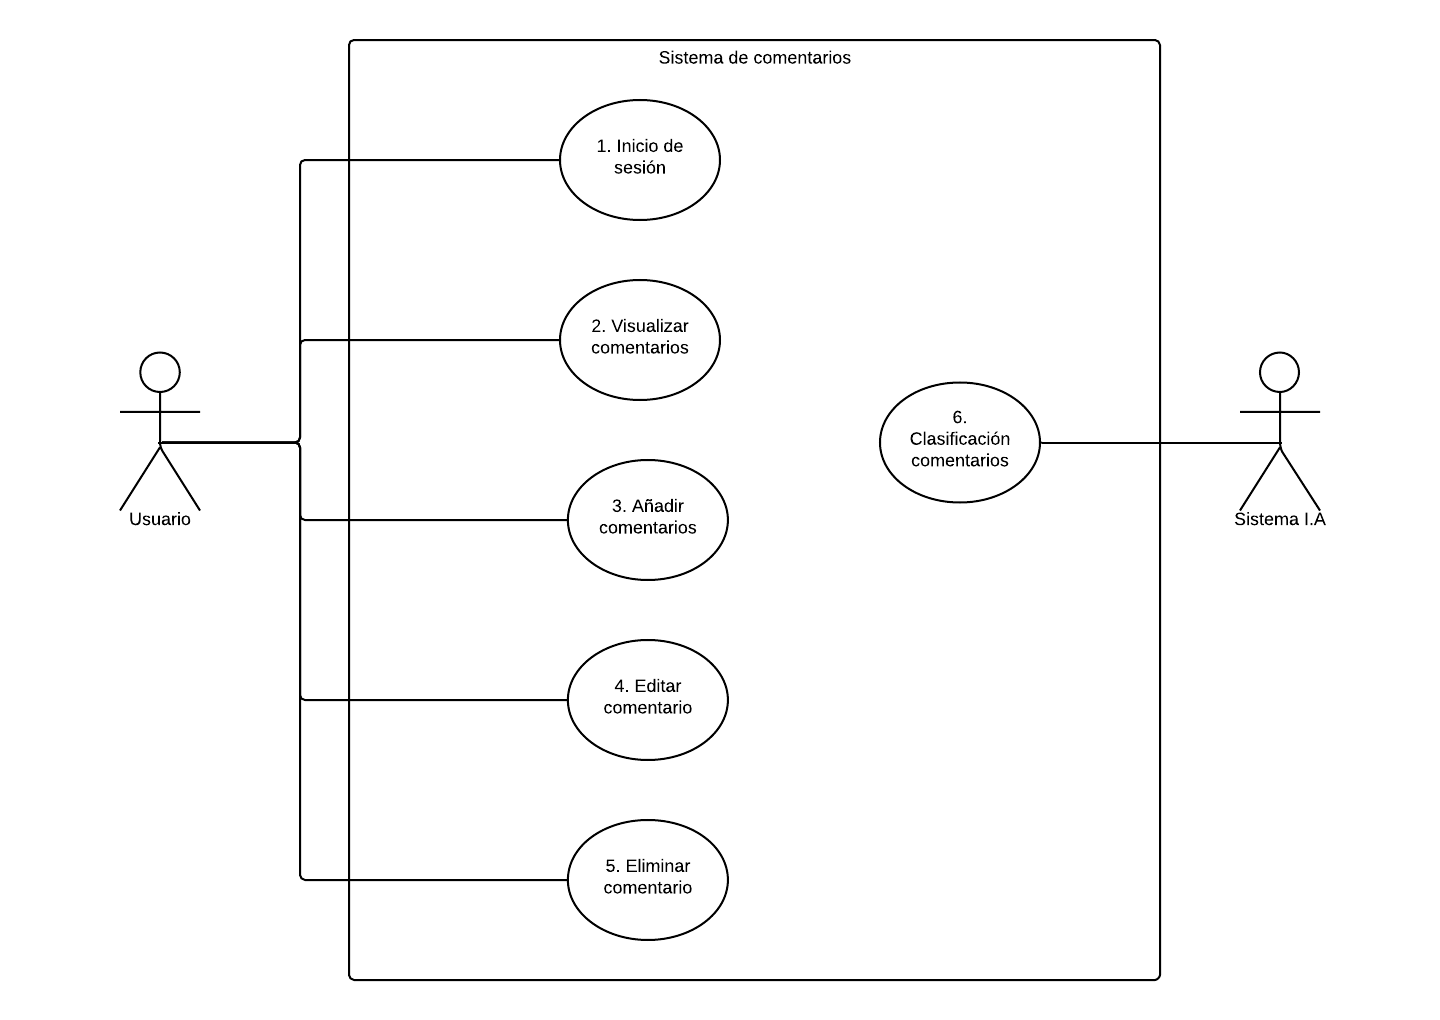
\includegraphics[width=1\textwidth]{imaxes/usecases.png}
	\caption{Casos de uso}
		\label{usecases}
\end{figure}

\section{Inicio de sesión}

\paragraph{Descripción} El usuario iniciará sesión en la aplicación introduciendo sus credenciales en un formulario.

\paragraph{Precondición} N/A

\paragraph{Secuencia} La secuencia de acciones será la siguiente:

\begin{itemize}
	\item El usuario pulsa el botón de inicio de sesión.
	\item El usuario introducirá el usuario y contraseña en el formulario.
	\item Si las credenciales son correctas se notifica al usuario de que su sesión se ha iniciado y se cambia el botón de inicio de sesión por el botón de gestión de perfil.
	\item Si las credenciales no son correctas se notifica al usuario y se vuelve a pedir que las introduzca de nuevo.
\end{itemize}

\paragraph{Postcondición} La sesión del usuario quedará iniciada en el sistema.

\section{Visualizar comentarios}

\paragraph{Descripción} El usuario visualizará los comentarios de un artículo cuando abra la ficha del mismo haciendo click sobre el mismo en la pantalla principal.

\paragraph{Precondición} N/A

\paragraph{Secuencia} El caso de uso comenzará cuando el usuario haga click sobre un artículo determinado en la rejilla de resultados de búsqueda.

\section{Añadir comentarios}

\paragraph{Descripción} El usuario podrá añadir comentarios relacionados con alguno de los artículos del sistema.

\paragraph{Precondición} El usuario debe estar registrado.

\paragraph{Secuencia} La secuencia de acciones será la siguiente:

\begin{itemize}
	\item 1 El usuario hace click sobre alguno de los artículos de la rejilla de resultados de la página principal.
	\item 2 El usuario introduce el comentario que desee en el cuadro de texto.
	\item 3 El usuario puede publicar o cancelar el comentario.
	\SubItem{3.1 Si el usuario introduce una puntuación para el artículo esta se le asigna al comentario.}
	\SubItem{3.2 Si el usuario no introduce una puntuación el artículo se guardará sin puntuación asociada, y se le asignará mediante un modelo de clasificación inteligente.}
	\SubItem{3.3 Si el usuario cancela el envío del comentario se terminará el caso de uso.}
\end{itemize}
	
\paragraph{Postcondición} El comentario quedará dado de alta en el sistema.


\section{Editar comentarios}

\paragraph{Descripción} El usuario podrá editar los comentarios realizados con anterioridad.

\paragraph{Precondición} 
\begin{itemize}
	\item El usuario debe estar registrado.
	\item El comentario a editar debe pertenecer al usuario.
\end{itemize}

\paragraph{Secuencia} La secuencia de acciones será la siguiente:

\begin{itemize}
	\item 1 El usuario hace click sobre alguno de los artículos de la rejilla de resultados de la página principal.
	\item 2 El usuario elige la opción de edición sobre uno de sus comentarios.
	\item 3 El usuario puede aplicar o cancelar la edición.
	\SubItem{3.1 Si el usuario introduce una puntuación para el artículo esta se le asigna al comentario.}
	\SubItem{3.2 Si el usuario no introduce una puntuación el artículo se guardará sin puntuación asociada, y se le asignará mediante un modelo de clasificación inteligente.}
	\SubItem{3.3 Si el usuario cancela el envío del comentario se terminará el caso de uso.}
\end{itemize}

\paragraph{Postcondición} El comentario quedará modificado en el sistema.


\section{Eliminar comentarios}

\paragraph{Descripción} El usuario podrá eliminar los comentarios realizados con anterioridad.

\paragraph{Precondición} 
\begin{itemize}
	\item El usuario debe estar registrado.
	\item El comentario a editar debe pertenecer al usuario.
\end{itemize}

\paragraph{Secuencia} La secuencia de acciones será la siguiente:

\begin{itemize}
	\item 1 El usuario hace click sobre alguno de los artículos de la rejilla de resultados de la página principal.
	\item 2 El usuario elige la opción de eliminar sobre uno de sus comentarios.
	\item 3 El sistema pedirá confirmación antes de realizar el borrado.
	\SubItem{3.1 Si el usuario acepta la eliminación se borrará el comentario del sistema.} 
	\SubItem{3.2 Si el usuario no confirma la eliminación se termina el caso de uso.}
\end{itemize}
	
\paragraph{Postcondición} El comentario quedará borrado del sistema.

\section{Clasificar comentarios}

\paragraph{Descripción} El sistema puntuará los nuevos comentarios según la opinión reflejada en los mismos.

\paragraph{Precondición} 
\begin{itemize}
	\item Hay nuevos comentarios en el sistema o hay un nuevo modelo de clasificación.
\end{itemize}

\paragraph{Secuencia} La secuencia de acciones será la siguiente:

\begin{itemize}
	\item 1 Si hay un nuevo modelo de clasificación:
	\SubItem{1.1 Se obtienen todos los comentarios.}
	\SubItem{1.2 Se clasifican los comentarios obtenidos.}
	\SubItem{1.3 Se actualiza la clasificación de los comentarios en el sistema.}
	\item 2 Si hay nuevos comentarios:
	\SubItem{2.1 Se obtienen los nuevos comentarios.}
	\SubItem{2.2 Se clasifican los comentarios obtenidos.}
	\SubItem{2.3 Se actualiza la clasificación de los comentarios en el sistema.}
\end{itemize}
	
\paragraph{Postcondición} Todos los comentarios tienen una clasificación asociada.
